\documentclass[a4paper, twocolumn]{ctexart}
\usepackage[left=2cm, right=2cm, top=2.5cm, bottom=2.2cm]{geometry}

\usepackage{fancyhdr}
\usepackage{graphicx, subfigure}
\usepackage{minted}
\setmonofont[]{Fira Code}
\usepackage[shortlabels]{enumitem}
\setenumerate{itemsep=0pt,partopsep=0pt,parsep=\parskip,topsep=0pt, itemindent=4em, leftmargin=0pt, listparindent=2em, label=(\arabic*)}
\setitemize{itemsep=0pt,partopsep=0pt,parsep=\parskip,topsep=5pt}
\setdescription{itemsep=0pt,partopsep=0pt,parsep=\parskip,topsep=5pt}

\usepackage[sort&compress]{gbt7714}
\usepackage{hyperref}
\hypersetup{unicode, colorlinks=true, linkcolor=black, urlcolor=black}
\usepackage{booktabs}


\begin{document}

\pagestyle{plain}

\ctexset{
    section = {
      format = \zihao{4}\heiti,
      beforeskip = {2ex},
      afterskip = {2ex}
     },
    subsection = {
            format = \zihao{5}\heiti,
            beforeskip = {2ex},
            afterskip = {1ex},
        },
    subsubsection = {
            format = \zihao{5}\songti,
            beforeskip = {2ex},
            afterskip = {1ex},
        },
    appendix = {
            name = {附录}
        }
}
\linespread{1}

\title{\textbf{超声测距系统的设计}}
\author{duskmoon314\textsuperscript{1},Phynon\textsuperscript{2}\\
{\small (1. \href{https://github.com/duskmoon314}{github/duskmoon314};2. \href{https://github.com/Phynon}{github/Phynon})}
}
\date{}
\maketitle

\thispagestyle{fancy}
\chead{电子电路课程设计(2)}
\lhead{}
\lfoot{
    \small{实验时间:9月10日-9月11日 \\ 实验地点:清华大学中央主楼903室}
}
\renewcommand{\headrulewidth}{1pt}

\setcounter{section}{-1}

\section{课程任务和实验要求}
\subsection{课程任务}
《电子电路课程设计》是一门综合应用模拟电路和数字电路理论进行电子系统设计的课程,要求设计并制作具有较完整功能的小型电子系统,它侧重于电子技术理论知识的灵活运用和设计的创新,因此具有系统性、综合性和探索性。课程任务有:
\begin{enumerate}
    \item 掌握一般电路系统的设计思路和方法
    \item 培养系统观念和工程观念、解决电路实际问题的能力和探索创新精神
    \item 培养实验研究的总结和表达能力
\end{enumerate}

\subsection{实验要求}

设计并制作一个超声测距系统。

\begin{enumerate}
    \item 基本要求:

          用示波器显示并测量出接收波与发射波的时延,计算出测量距离。

          测量距离大于1m,显示精度为0.01m,数字显示测量结果,并能动态更新。

          测量距离大于2m,显示方式同上。

    \item 提高要求:

          实现测量距离的稳定显示,即显示不闪烁。
\end{enumerate}



\section{实验设计}
\subsection{总体方案设计}
此超声测距系统基于分为三个部分:
\begin{enumerate}
    \item 40kHz窄脉冲的放大与发射;
    \item 超声波信号的接收、放大、整形与数字化;
    \item 时钟生成、脉冲信号调制、计数与显示。
\end{enumerate}

前两个部分需进行模拟电路设计,第三个部分则需进行数字电路的设计。考虑到硬件的可靠性,我们使用 Verilog 硬件描述语言和基于 Xilinx Artix 7 FPGA 的 EGO1 开发板进行第三部分的设计,使用直插式LF347和CD40106等器件进行前两个部分的设计。

测距系统的工作流程为:

\begin{enumerate}
    \item FPGA产生受34Hz窄脉冲调制的40kHz方波,同时开始以17kHz的频率计数;
    \item 放大调制波并使用超声波发射装置发射;
    \item 接收返回的超声波,放大、数字化并整形,输入FPGA;
    \item FPGA检测到信号前沿,暂停计数,寄存计数并显示;
    \item 下一个34Hz到来时回到1,重复所有步骤。
\end{enumerate}

使用17kHz进行计数,计数结果为以1cm为分度的测距结果,满足精度要求。使用34Hz作为每次测量步骤的起始点,保证可以使用17kHz计数从0到499,即量程可达5m,满足量程要求。

\subsection{电路框图设计}

电路的整体设计框图如图\ref{fig:block_sch}所示。其中中间虚线表示FPGA,用于实现总体方案设计中部分(3)。其上方为超声波发射部分,下方为超声波接受部分,分别对应于总体方案设计的部分(1)和部分(2)。

\begin{figure}[ht]
    \centering
    
\includegraphics[width=7.5cm]{../assets/系统框图.png}
    \caption{电路框图}
    \label{fig:block_sch}
\end{figure}

\subsection{数字电路设计}

如总体设计所述,本实验为保证硬件的可靠性,使用Verilog硬件描述语言FPGA开发板实现时钟生成、信号调制、计数与显示等功能,并将关键接口通过板上引脚与外围电路连接,完成整体设计。数字电路部分原理图见图2,Verilog代码与约束文件见附件。下面分模块进行介绍。

\begin{figure}[ht]
    \centering
    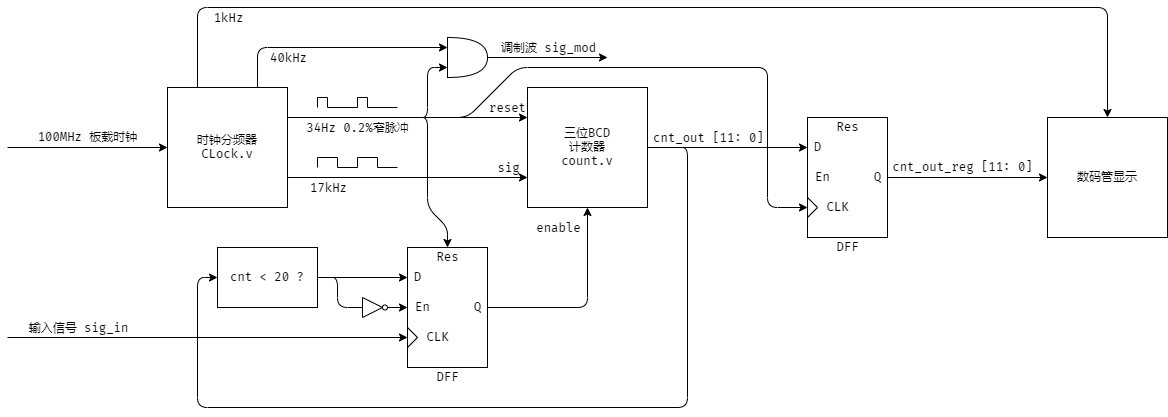
\includegraphics[width=7.5cm]{../assets/数字电路原理图.png}
    \caption{数字电路原理图}
    \label{fig:digital_sch}
\end{figure}

\subsubsection{时钟生成于信号调制模块}

如总体设计所述,本实验需要 40kHz、17kHz、1kHz 时钟和 34Hz 窄脉冲。使用 FPGA 板载 100MHz 时钟,并结合计数分频,生成周期为 25$\mu$s、58.82$\mu$s、1ms 的方波,即 40kHz、17.001kHz(误差很小,下称为 17kHz 时钟)、1kHz 的时钟。再对 17kHz 时钟进行计数分频,生成占空比 0.2\%的 34Hz 窄脉冲。后文中分别称这些信号为 clk\_40k、clk\_17k、clk\_1k 和 clk\_34。

调制信号为窄脉冲时间段内的 40kHz 方波,故使用 clk\_40k 和 clk\_34 直接通过二输入与门得到,再通过板上针脚引出。

时钟模块仿真验证如下,上升沿间距分别为58.82$\mu$s和29.41ms,证明设计正确:

\begin{figure}[ht]
    \centering
    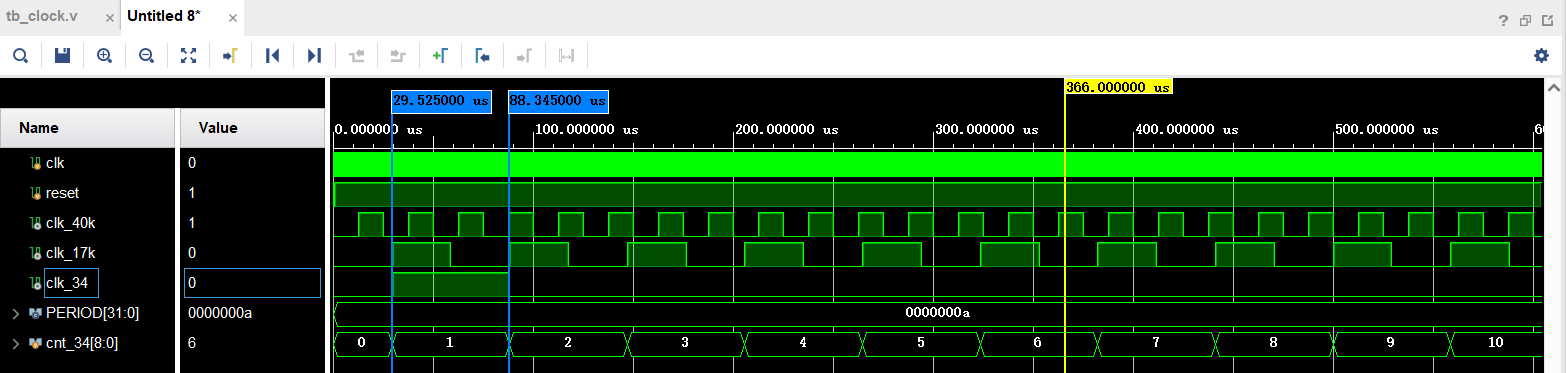
\includegraphics[width=7.5cm]{../assets/clock_17k.png}
    \caption{17kHz时钟仿真波形}
    \label{fig:sim_clk_17k}
\end{figure}

\begin{figure}[ht]
    \centering
    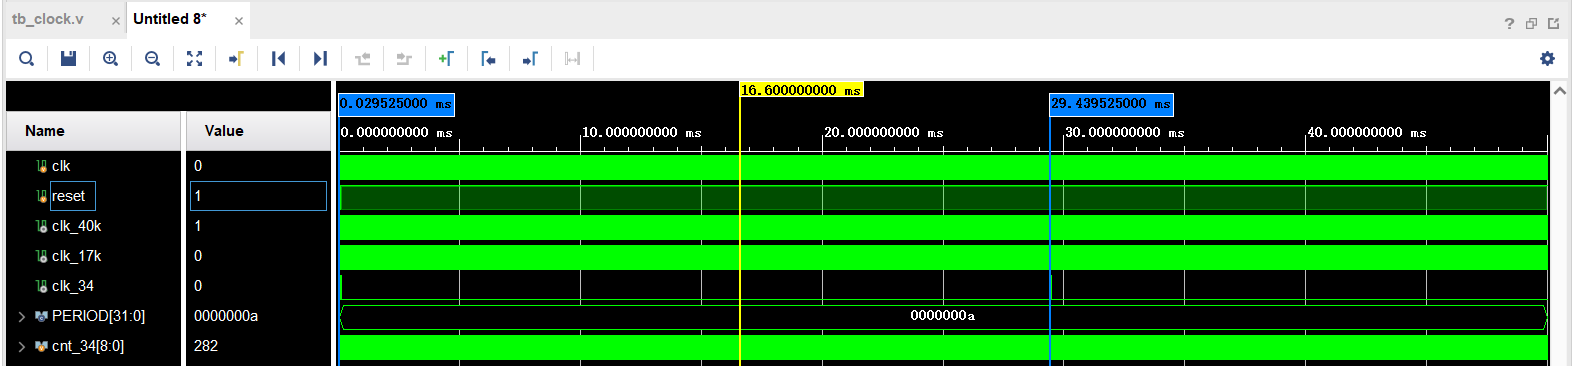
\includegraphics[width=7.5cm]{../assets/clock_34.png}
    \caption{34Hz窄脉冲仿真波形}
    \label{fig:sim_clk_34}
\end{figure}

\subsubsection{计数模块}

由于需要对计数和信号发射进行控制,计数器需要一个复位信号、一个使能信号以及计数信号和输出信号接口。实验中使用 clk\_34 作为复位信号,当 clk\_34 上升沿到来时将计数器复位为 0,并将使能信号 enable 置为 1,开始对 clk\_17k 进行计数。当超声波接收装置接收到回波的信号经外围电路处理后传入 FPGA,会先使用逻辑判断此时计数是否大于等于 20,如果为是则将 enable 拉低为 0,停止计数器计数。输出信号为 12 位 BCD 码,满足 clk\_34 对应计数 0-499 的需要,即量程为 5m,精度 0.01m。

是否大于 20 的判断是本检测器的死区设置。根据实验的观察,超声波发射装置发射的信号会直接传到接收装置中,这个干扰信号距离信号发送时间基本在 1ms 以内,故添加死区以排除干扰。

\subsubsection{显示模块}

本实验使用 FPGA 板上 7 位数码管进行显示。由于计数器输出为 12 位 BCD 码,显示部分需要将其转为 7 位数码管控制信号,在每次 clk\_34 的上升沿到时将前一个周期的计数结果存在寄存器后使用组合逻辑转为控制信号进行显示。由于使用的 FPGA 板的数码管间不独立,使用 1kHz 时钟对三个数码管进行扫描显示。

\subsection{数字电路仿真分析}

为确认Verilog代码与设计功能相一致,我们利用Vivado的仿真功能,结合如下代码进行测试:

\begin{minted}{verilog}
  always @( posedge clk )
    begin
      sig_in <= #2058823 sig_mod;
    end
\end{minted}

即将FPGA生成的调制信号延时2058823ns后传入信号接收端口,用来测试是否能正确显示34。仿真得到波形如图\ref{fig:digital_sim}。

\begin{figure}[ht]
    \centering
    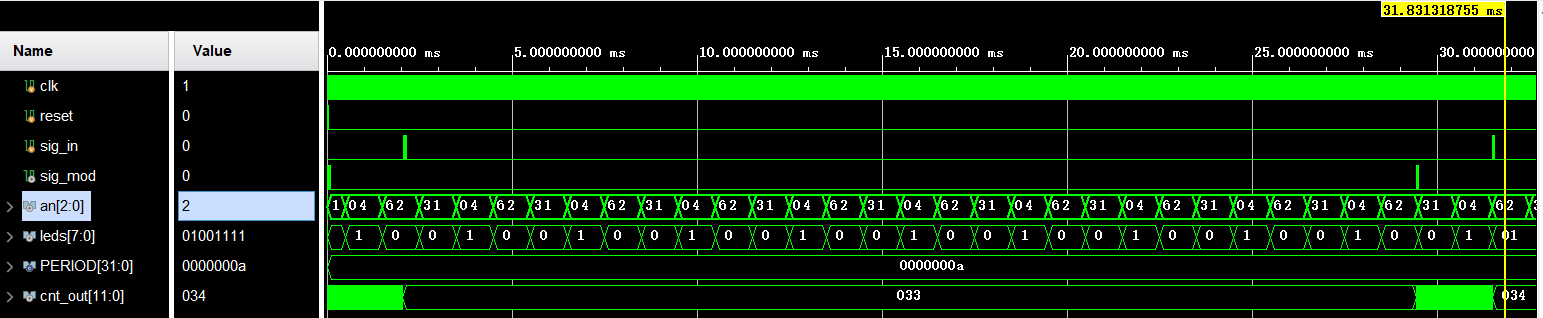
\includegraphics[width=7.5cm]{../assets/仿真.png}
    \caption{数字电路仿真波形}
    \label{fig:digital_sim}
\end{figure}

由于刚上电时的复位信号,导致第一次发射调制信号前有一小段未定状态信号,故第一个运行周期少计一次为33,之后正常计数得到34。传输给板上数码管的信号也符合033对应的10111111\_01001111\_01001111(最高位为小数点控制信号),功能正常。

通过仿真,我们确认代码与设计功能相符,各部分均符合预期在理想的信号条件下正常工作。

\subsection{模拟电路设计}

根据框图,整个设计的模拟电路分为发射机和接收机两个部分。

发射机接受从FPGA传来的窄脉冲输入,将窄脉冲信号放大后送入扬声器,扬声器将电信号转化为超声信号,发送到大气中。

接收机的传感器将拾音得到的超声信号直接变为电信号,输入给后面的放大电路。信号经两级反相放大后,信号与一个参考电平作比较,以滤去大部分噪声,再经电平匹配和整形,压限成FPGA可接受的幅值,再送入FPGA,进行后续的检测和计数处理。

\subsubsection{超声波发射电路}

由于调制好的窄脉冲已经由FPGA产生,发射电路相对来说就比较简单。为方便起见,使用LF347构建同相比例放大电路,放大倍数一开始定为2倍,在完成了电路的功能测试之后,又进行优化,增大到3倍。

\subsubsection{超声波接收电路}

传感器直接产生的电信号幅值在mV量级,频率为40kHz。放大电路可以采用反相放大和同相放大两种设计,由于传感器没有直流通路,采用同相放大就必须额外增加运放的直流通路。考虑到运放摆率的问题,我们的放大电路采用LF347实现。LF347的增益带宽积为4MHz,因此每级比例放大的倍数不能超过100倍。根据课程资料提供的放大电路设计方案,我们采用两级反相放大,每级的放大倍数为100倍,两级放大电路之间设置一个交流耦合电容,容值需要视情况选取合适的值。电压比较器仍然使用LF347同两个限流电阻构造而成,参考电平由某个固定电压经电位器分压而产生,可以根据实验中的具体情况来调节。我们使用一个限流电阻和两个CD40106反相器构造电平匹配和整形电路,CD40106的供电电压由FPGA开发板自带的3.3V电源提供,从根本上避免了输出信号电平过高烧坏FPGA的可能性。信号经过两个反相器之后被量化,可以认为是实现了模拟转为数字。

\subsection{模拟电路仿真分析}

\subsubsection{发射电路仿真分析}

在设计时,按照发射电路放大倍数为2倍进行仿真。Multisim不方便接入直接调制好的短脉冲,因此信号源采用了两个方波相与的形式进行实现。如果不用FPGA,则这应该也是实际电路的信号源的一个实现。根据信号源V2的占空比,短脉冲当中,应有2个或3个上升沿。

\begin{figure}[ht]
    \centering
    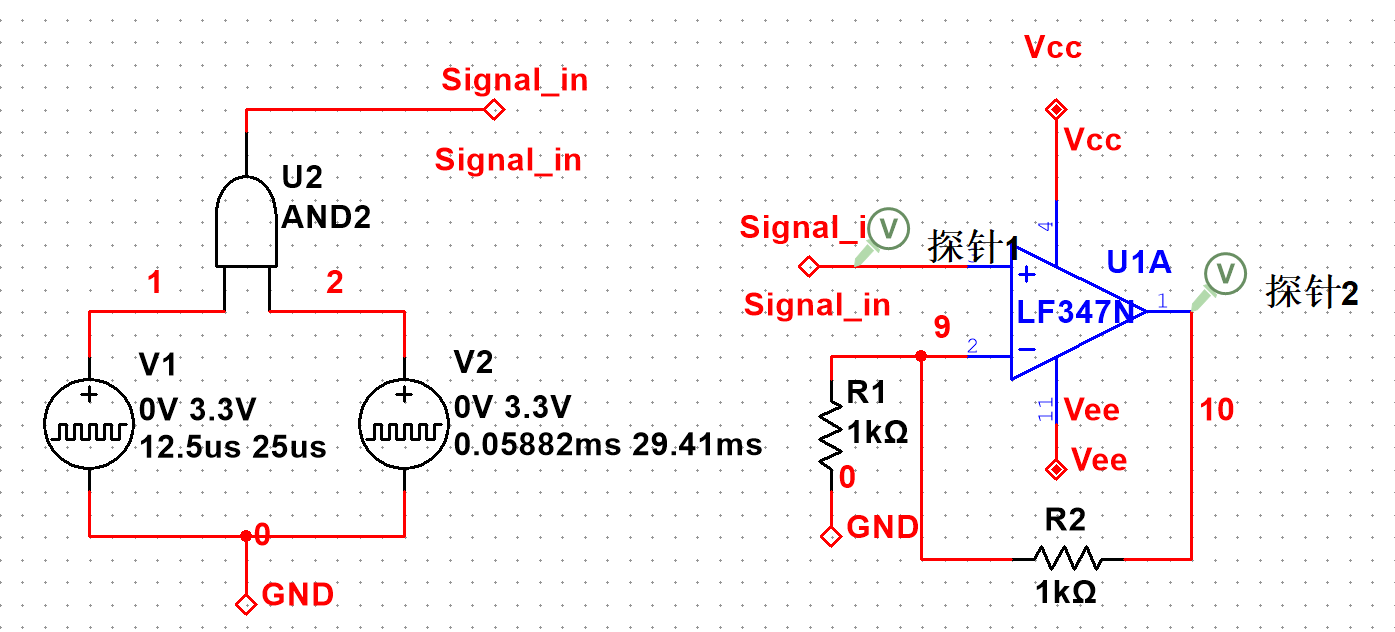
\includegraphics[width=7.5cm]{../assets/发射电路仿真原理图.png}
    \caption{发射电路仿真原理图}
    \label{fig:tran_sim_sch}
\end{figure}

仿真的结果如图\ref{fig:tran_sim_result}所示。这一段短脉冲有3个上升沿,放大后得到的输出信号存在一定的上升时间,长得像一串梯形波,说明LF347的摆率虽高,也并不能称之为理想。

\begin{figure}[ht]
    \centering
    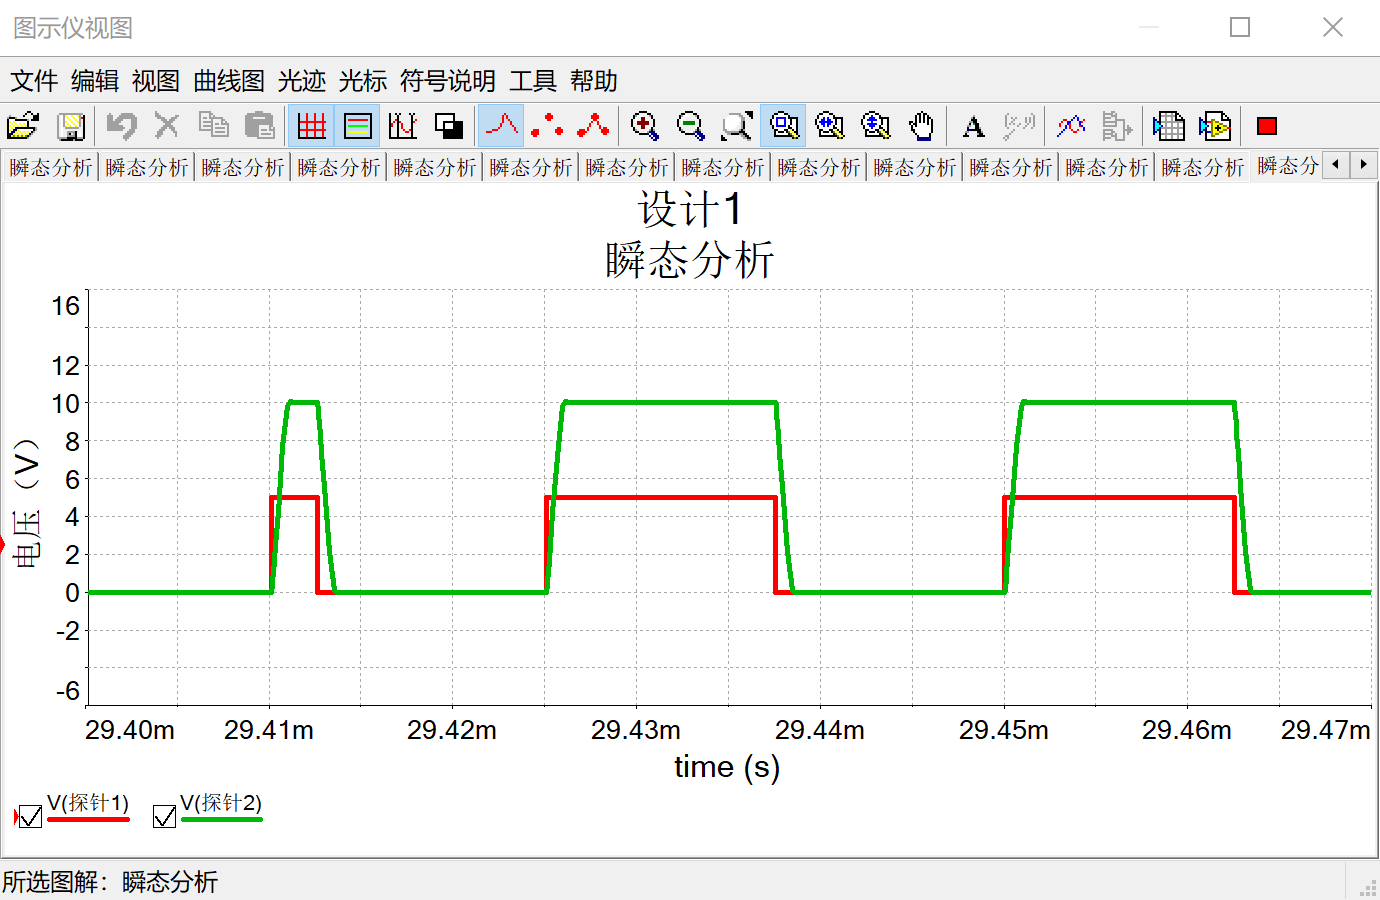
\includegraphics[width=7.5cm]{../assets/发射电路仿真结果.png}
    \caption{发射电路仿真结果}
    \label{fig:tran_sim_result}
\end{figure}

\subsubsection{接收电路仿真分析}

接收电路的部分,相对来说较为复杂。超声波传感器的输出约为mV量级,我们为了模拟这个信号,在Multisim中加入了一个幅值为1mV,频率为40kHz的方波作为待接收的信号。同时,为了模拟环境中超声噪声对信号接收的影响,我们还添加了一个热噪声源,一同输入到接收电路当中。两级放大电路按照设计值进行搭建,两级之间的耦合电容起隔直流、通交流的作用,应当选择较大的电容。同样是由于仿真软件的部分限制,电压比较器的参考电压使用了两个可变电阻分压VDD产生,相当于使用了单个电位器。仿真当中的CD40106电源电压只能选取为5V,在实际实验时,应从FPGA接出一个3.3V的电平为CD40106供电。

\begin{figure}[ht]
    \centering
    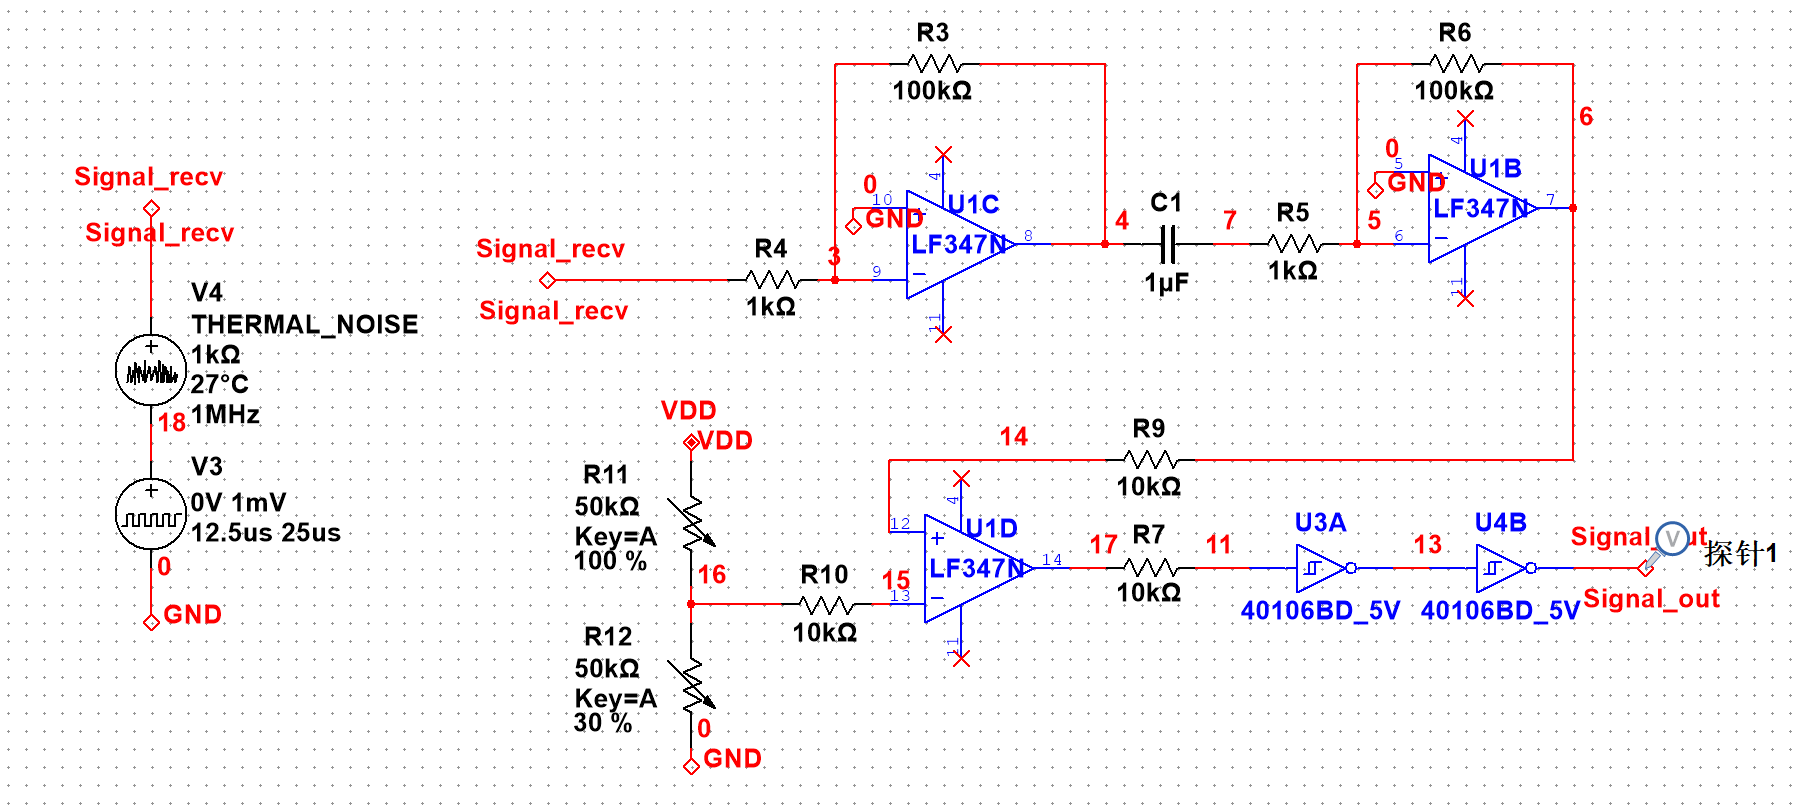
\includegraphics[width=7.5cm]{../assets/接收电路仿真原理图.png}
    \caption{接收电路仿真原理图}
    \label{fig:rec_sim_sch}
\end{figure}

经过两级放大之后,输出的信号波形仿真如图\ref{fig:rec_sim_amp}。由于1$\mu$F的电容容值相对不是很大,因此两级放大后的输出幅值也没有达到输入信号的10000倍。继续增大电容容值,刚上电时电容充电产生的延时就会增加,电路需要较长的时间才能进入正常工作状态。为了确认较好的电容容值,我们进行了多次仿真,最终实验时采用了一个10$\mu$F的电容。

\begin{figure}[h]
    \centering
    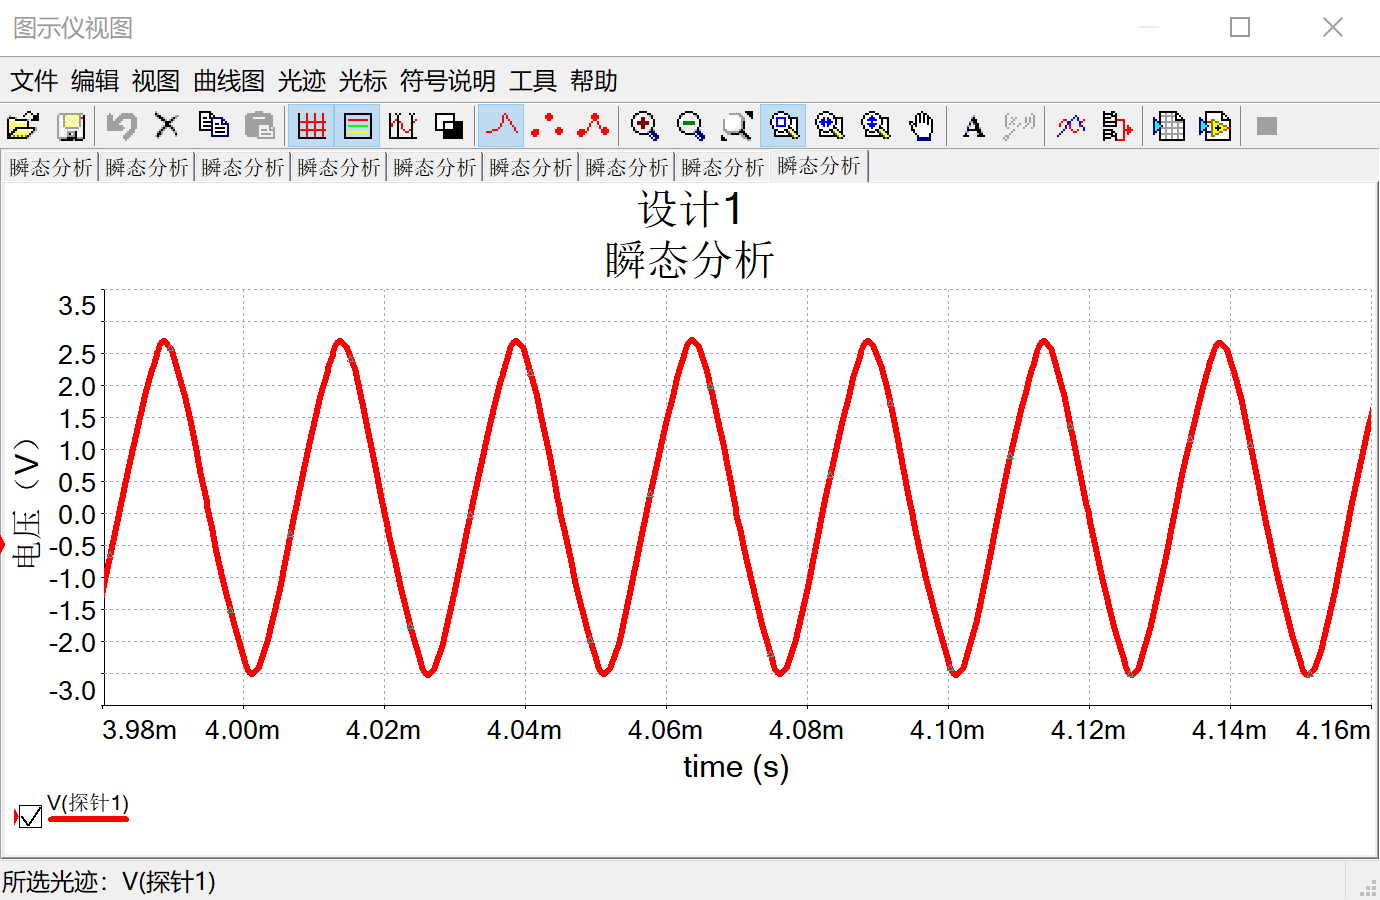
\includegraphics[width=7.5cm]{../assets/两级放大仿真波形.png}
    \caption{两级放大仿真波形}
    \label{fig:rec_sim_amp}
\end{figure}

电压比较、匹配和整形后的仿真波形如图\ref{fig:rec_sim_CD40106}所示。经过高速非门之后,信号的上升时间和下降时间均可忽略不计,两个上升沿之间相距约为25$\mu$s,信号的最低电平为0,最高电平为CD40106的供电电压5V。FPGA检测波形前沿时关心的两个最关键的部分都没有问题,这证明了放大器后级去噪和数字化电路设计是正确的。

\begin{figure}[h]
    \centering
    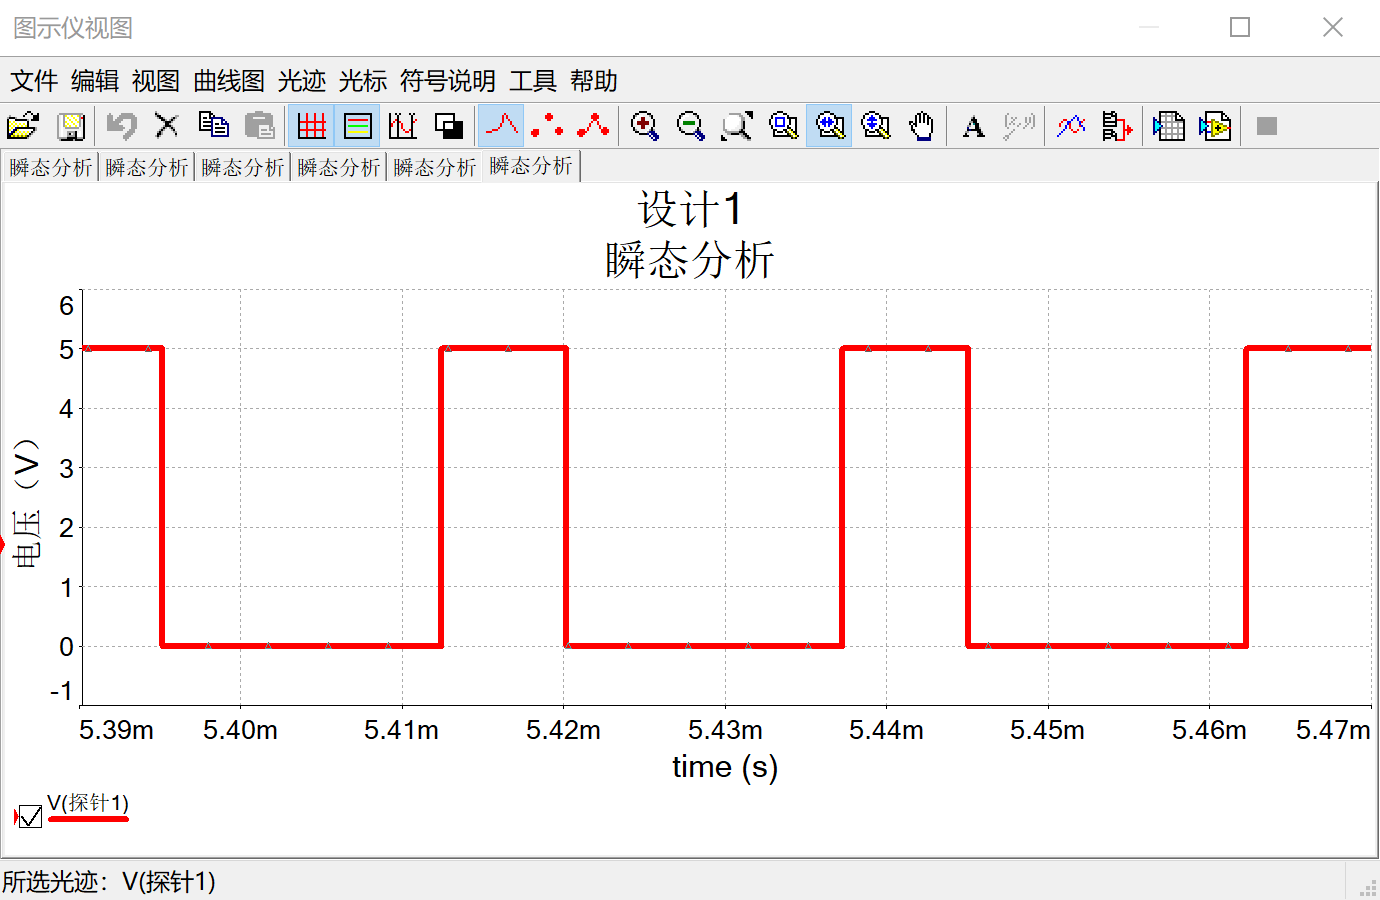
\includegraphics[width=7.5cm]{../assets/匹配整形仿真波形.png}
    \caption{匹配整形仿真波形}
    \label{fig:rec_sim_CD40106}
\end{figure}

\subsubsection{关键元器件作用说明}

\begin{itemize}
    \item LF347:一个集成块上集成了4个放大器,其中1个用作发射的驱动放大器,2个用作接收端的两级放大,另外1个用来搭建电压比较器电路。

    \item 放大电路当中的反馈电阻:对于同相放大器,放大倍数$A=\frac{R_2+R_1}{R_1}$;对于反相放大器,放大倍数$A=\frac{R_2}{R_1}$。依照这两个公式确定3个放大电路的电阻阻值。

    \item 耦合电容:在接收端,使交流信号从第一级放大通到第二级放大。经过多次仿真测试,这个电容的容值在1$\mu$F到100$\mu$F之间为宜。如果太小,对信号的容抗会很大,交流信号很难通过;如果太大,上电时的延时会很高,电路需要较长时间才能进入正常工作状态,不过这一问题可以通过适当调整后级比较器的参考电平来解决。实验中使用的容值为10$\mu$F,收到了预期的效果。

    \item 电位器:靠分压调整比较器的参考电平,以滤去幅值较小的环境噪声。参考电平过低,则噪声滤不掉;参考电平过高,则会把信号和噪声一起滤掉。因此,电位器必须根据实际情况适当调整,做到既能滤去噪声,又不把回波信号也滤掉。

\end{itemize}

\section{实验数据整理和分析}

\subsection{电路各关键节点波形}

使用上述系统进行实验时,我们使用示波器观察各关键节点,以确认系统工作正确与否。下面仍按数字电路、模拟电路超声波发射部分、模拟电路超声波接收部分逐个进行分析。

\subsubsection{数字电路波形分析}

数字电路对外仅暴露经34Hz窄脉冲调制后的40kHz方波。示波器测量输出波形如图\ref{fig:clk_34_real}。

\begin{figure}[ht]
    \centering
    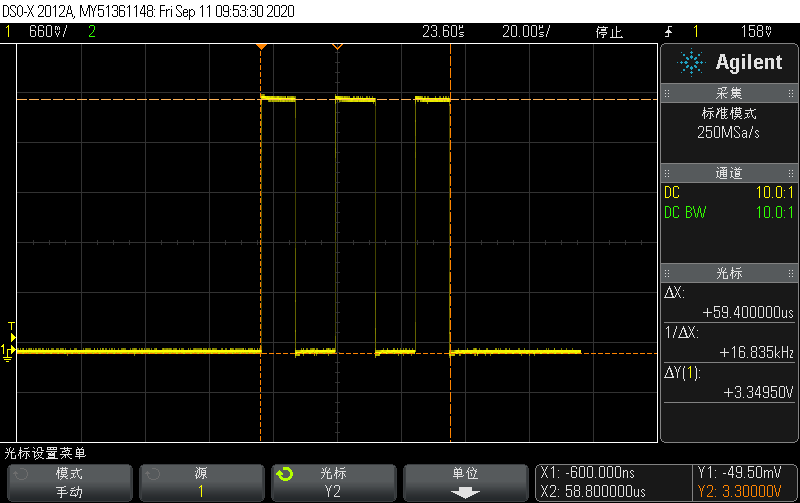
\includegraphics[width=7.5cm]{../assets/trans_2.png}
    \caption{34Hz窄脉冲调制40kHz波形}
    \label{fig:clk_34_real}
\end{figure}

根据测量结果,脉冲仅存在约59$\mu$s,对应34Hz整个周期的0.2\%,也即17kHz的一个周期。脉冲的频率亦可测量确认为40kHz。故得到的波形符合设计。

\subsubsection{模拟电路超声波发射部分}

模拟电路超声波发射部分主要将数字电路输出的波形进行放大,其波形见图\ref{fig:tran_amp}。

\begin{figure}[ht]
    \centering
    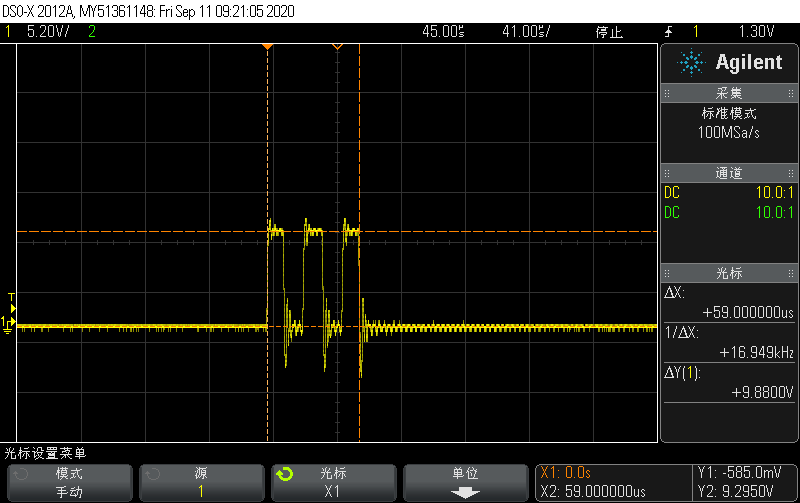
\includegraphics[width=7.5cm]{../assets/trans_1.png}
    \caption{发射放大电路输出波形}
    \label{fig:tran_amp}
\end{figure}

如图\ref{fig:tran_amp}所示,波形经放大电路后放大了2.9497倍,与设计的放大3倍相符,接近运放的饱和电压。

注意到图中有较强的振铃,波形不很理想。这个振铃主要是超声波发射装置带来的,去掉装置后波形接近标准的矩形波。推测装置中的压电陶瓷不允许高频信号通过,从而让波形表现出振铃。

\subsubsection{模拟电路超声波接收部分}

本实验中,接收电路的关键节点有两级级放大、数字化和整形,目的在于将模拟信号转化为合适的数字信号供FPGA进行处理。下面使用障碍物在平放在桌面的系统上方65cm处的波形进行验证,理论计算啊易得回波前沿应距离发射3.82ms。

\begin{figure}[ht]
    \centering
    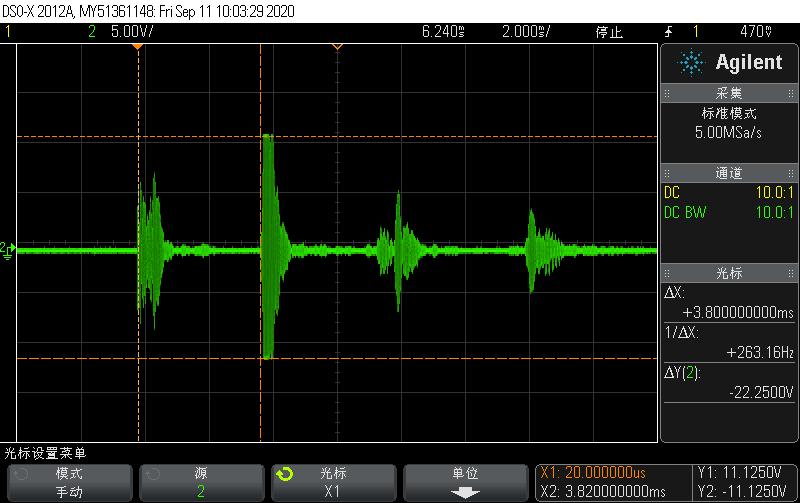
\includegraphics[width=7.5cm]{../assets/recv10k_65.png}
    \caption{两级放大后的接收信号}
    \label{fig:rec_10k_amp}
\end{figure}

\begin{figure}[ht]
    \centering
    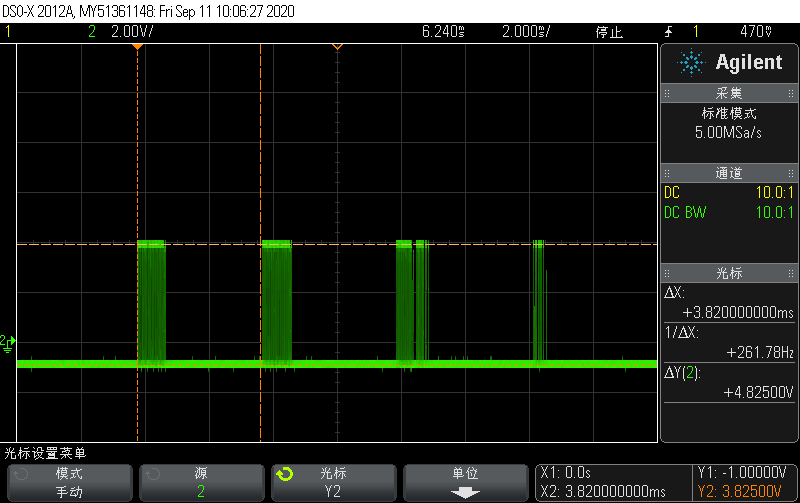
\includegraphics[width=7.5cm]{../assets/recvcomp_65.png}
    \caption{电压比较器输出信号}
    \label{fig:rec_cmp}
\end{figure}

图\ref{fig:rec_10k_amp}为接收信号经两级放大后的波形,图\ref{fig:rec_cmp}为经电压比较器进行数字化后波形,可以看到总共有四段脉冲波形,初步判断分别是直接来自发射装置、经障碍物反射、经障碍物和桌面三次反射、天花板反射。

经两级放大后,最主要的回波信号幅度已达到运放输出的饱和电压,且不存在除了推测来自发射装置的信号外的噪声信号,符合设计要求。经过电压比较器后,信号被数字化为高电平5V的方波信号,噪声信号被滤去,符合设计要求。实验中我们得到电压比较器的参考电压在0.5-0.7V比较合适,过小的比较电压无法除去噪声,过大的比较电压会将距离远的回波信号滤去从而降低量程。

\begin{figure}[ht]
    \centering
    \subfigure[经障碍物一次反射]{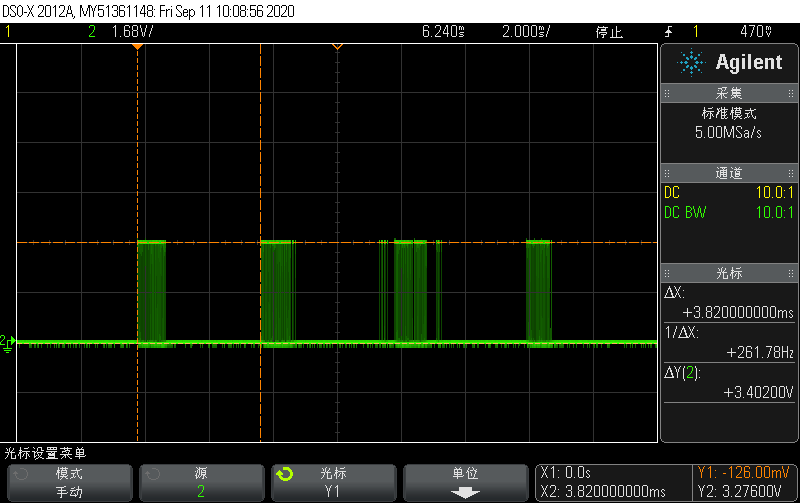
\includegraphics[width=7.5cm]{../assets/recv40106_65.png}}
    \subfigure[经障碍物和桌面三次反射]{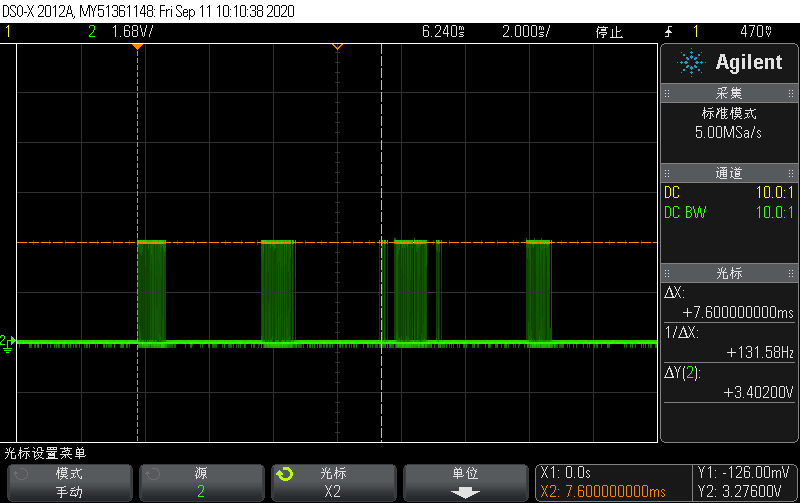
\includegraphics[width=7.5cm]{../assets/recv40106_65_2nd.png}}
    \subfigure[天花板反射]{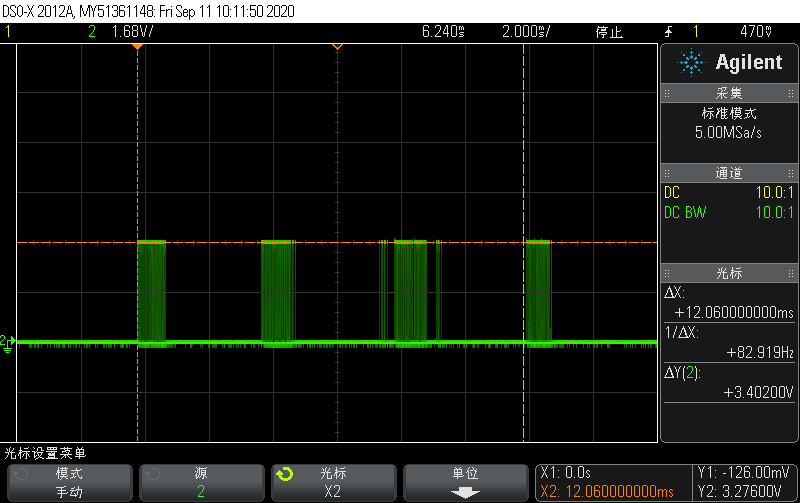
\includegraphics[width=7.5cm]{../assets/recv40106_65_ceil.png}}
    \caption{CD40106整形后输出信号}
    \label{fig:rec_40106}
\end{figure}

图\ref{fig:rec_40106}为经CD40106整形后输出给FPGA的信号。我们使用FPGA板上3.3V和GND接口给CD40106进行供电,从而得到适合输入的波形并保护FPGA。实验测量得到输出波形幅值3.4V,矩形波清晰没有噪声,满足设计要求。

可以看到,后面三段脉冲的最前沿距离发射时间分别为3.82ms、7.6ms、12.06ms,换算为距离得到64.94cm、129.2cm、205.02cm,恰好是装置到障碍物的距离、装置到障碍物的距离的两倍、装置到天花板的距离,与上面的判断一致。最前面的脉冲推测为直接来自发射装置,其存在时间约为1ms,对应障碍物据系统约17cm,故设计中的死区设置为20cm是合适的。

\subsection{不同距离测量情况}

为验证系统的量程涵盖20cm-2m的范围,我们使用记录FPGA板上数码管示数、人工测量、示波器测量换算的方法对30cm、60cm、90cm、120cm、桌面到天花板(减去系统高度后为2.02m)进行测试。结果记录于表\ref{tab:dis_result}。部分测试的示波器波形见图\ref{fig:dis_result_osc}。

\begin{table}[ht]
    \centering
    \caption{不同距离超声波测距结果}
    \label{tab:dis_result}
    \begin{tabular}{cccc}
        \toprule
        实际(cm) & 延时(ms) & 换算(cm) & 示数(cm) \\
        \midrule
        30       & 1.8      & 30.6     & 30       \\
        60       & 3.58     & 60.86    & 60       \\
        90       & 5.3      & 90.1     & 90       \\
        120      & 7.04     & 119.68   & 119      \\
        202      & 11.9     & 202.3    & 202      \\
        \bottomrule
    \end{tabular}
\end{table}

\begin{figure}[ht]
    \centering
    \subfigure[30cm]{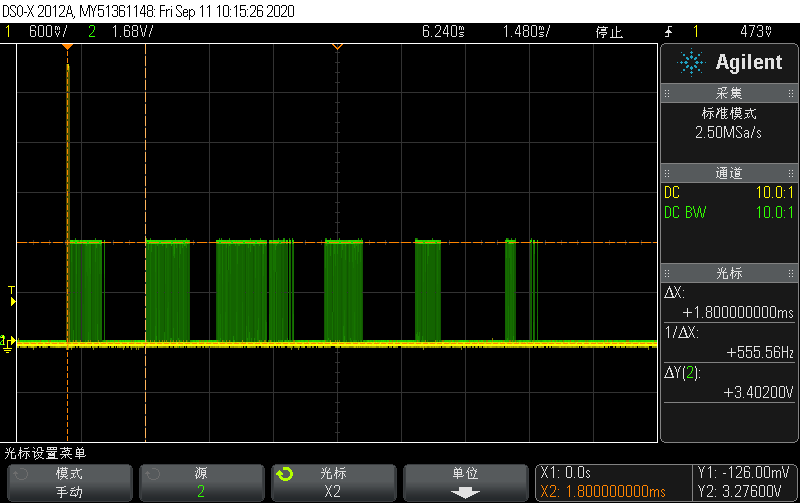
\includegraphics[width=7.5cm]{../assets/30cm.png}}
    \subfigure[60cm]{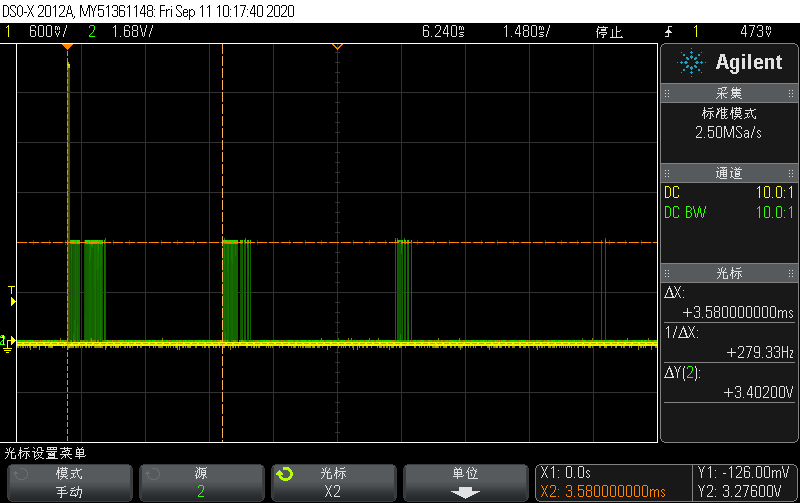
\includegraphics[width=7.5cm]{../assets/60cm.png}}
    \subfigure[90cm]{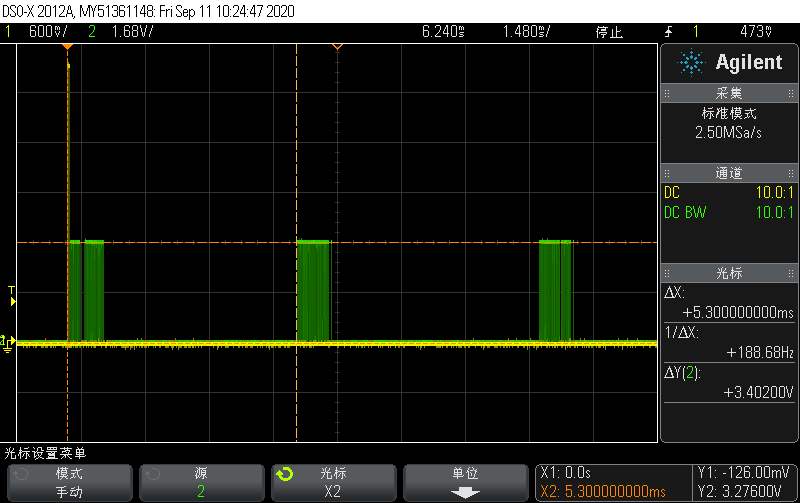
\includegraphics[width=7.5cm]{../assets/90cm.png}}
    \caption{部分距离测试示波器波形}
    \label{fig:dis_result_osc}
\end{figure}

表中的实际距离为人工使用卷尺测量,由于测试时系统放于桌面,障碍物由人握住保持在发射与接收器正上方,可能存在1cm左右的误差。表中的延时和换算对应示波器测量波形得到的回波前沿与发射脉冲的距离。示数为FPGA板上数码管显示的数字换算为以cm单位后的数据。示波器测量延时进行换算采用方式为:使用游标测量延时$\Delta_t$(ms),然后计算$d = \frac{340 \Delta_t}{2}$(mm)。

总体上,示数与实际距离偏差较小,系统在设计的量程范围内正常工作。但由于测量时障碍物的实际距离与人工测量存在偏差,故实际距离和示数间存在约$\pm$1cm的误差。

为了测试系统的有效量程,我们将系统放置与地面,尝试测试水平发射和竖直发射测试天花板距离两种情况。由于实验室水平发射超声波易受桌椅和其他同学的干扰,在2.5m以外较难调试,我们最终竖直发射测得收发装置据天花板为2.81m,装置示数见图\ref{fig:ceil}。基本上在2.8m的范围内,系统都能准确显示,但越远越容易受到干扰,造成短时间内的示数错误。

\begin{figure}[ht]
    \centering
    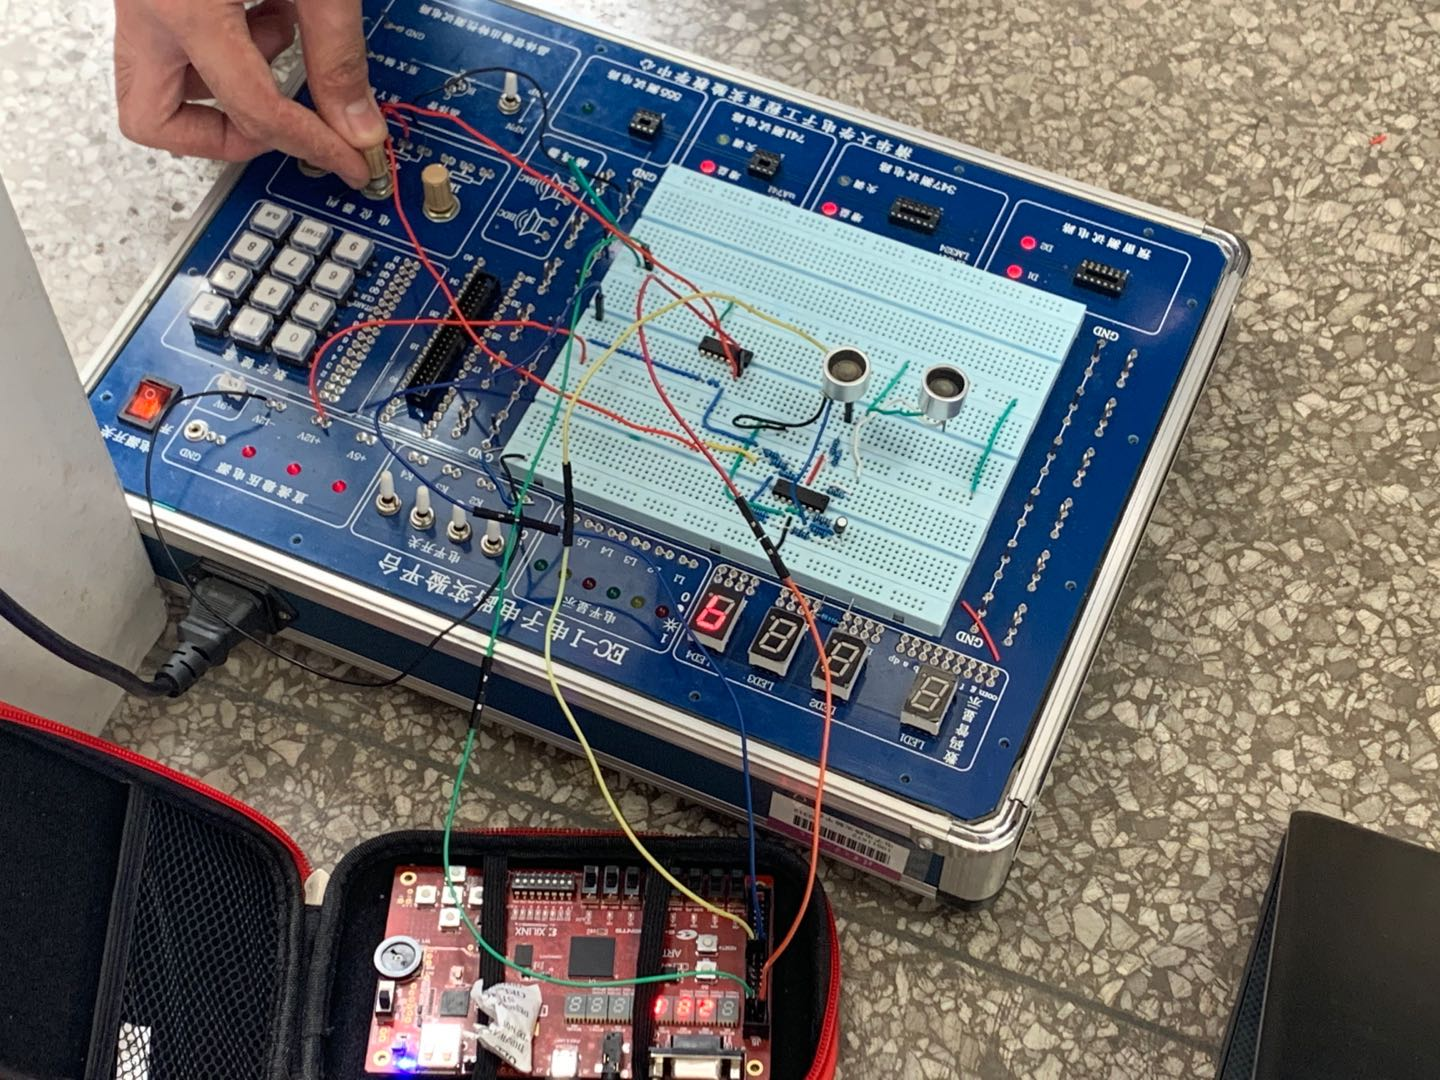
\includegraphics[width=7.5cm]{../assets/量程测试.jpg}
    \caption{量程测试时装置}
    \label{fig:ceil}
\end{figure}

\subsection{系统误差分析}

我们设计的超声测距系统虽然实验结果比较理想,但仍存在一些误差,导致部分情况下最后一位示数存在闪烁的现象。总体来看,误差可以分为电路设计引入的误差和测距时人工操作引入的误差。

电路设计上,有如下误差:

\begin{enumerate}
    \item 发射的受34Hz窄脉冲调制的40kHz方波并不一定在clk\_34的上升沿发出,而是可能延后最多12.5$\mu$s,即clk\_34的上升沿时clk\_40k恰为低电平。故计数结果存在一定的偶然误差;
    \item 计数器按照给定的clk\_17k时钟进行离散计数,而非连续测量,这是系统误差;
    \item 电路各部分存在时延,实际发射和接收的时间差会略小于系统测量的时间,这是电路系统的系统误差;
    \item 电路使用的实验平台电位器似乎存在老化问题,导致电压比较器的参考电压偶尔出现一瞬的不稳。
\end{enumerate}

人工操作引入如下误差:

\begin{enumerate}
    \item 发射和接收装置不在同一水平面带来的系统误差;
    \item 发射和接收装置不正对障碍物带来的系统误差;
    \item 验证系统正确性时人工测量障碍物与装置距离的偶然误差;
    \item 测量时障碍物位置不确定引入的偶然误差。
\end{enumerate}

\section{实验总结}

\subsection{实验完成情况}

实验耗时一天半,测量距离为20cm-2.8m,精度0.01m,FPGA示数约30ms更新一次,稳定无闪烁,达到提高要求。系统经助教验收合格。

\subsection{设计问题}

\begin{enumerate}
    \item 测试时部分场景下接收不到回波。

          在系统的全部功能已经完成,进行测试时,我们使用实验平台的盖子做障碍物,上下移动来调整障碍物同系统间的距离。在距离小于1m时,系统的示数能够正常显示;在距离超过1m时,系统大部分时间之内常显2.03m的示数。这说明系统并未接收到障碍物反射来的回波,接入示波器观察和测试,也并未看到回波波形。经过一段时间的排查,我们最终发现,系统接收不到回波的原因是,手持障碍物移动到一定距离后,目测不准,与系统测距的方向偏斜过大,发射波根本没有打在障碍物上,系统自然只能接收到天花板反射的回波。

          解决办法:在之后的测试中,我们小心移动障碍物,确保障碍物一直在系统测距的方向上移动,解决了这个问题。

    \item 示数剧烈闪动。

          在模拟电路部分搭好,首次将输入信号接入FPGA时,我们发现用来显示示数的数码管所有位均在不停地剧烈闪动。无论障碍物距离系统远近,系统的显示都有问题,根本无法正常读出示数。不过,在移动障碍物的过程当中,我们观察到:障碍物移动大约0.1m,不断闪动的示数随之发生了10次抖动。这一现象说明,烧入FPGA的程序计数部分没有问题,仅仅是数显存在问题。同时,我们请教了孙忆南老师,孙老师一眼就推定了是数码管显示部分出了问题,让我们对老师多年以来积累的经验有了新的认识。

          解决办法:我们将逐位扫描数码管的时钟频率从10MHz降到1kHz,同时修改了显示的逻辑。我们原本设置了一个寄存器,用来缓存显示的内容,而复位时产生的0也会持续不断地写入其中,导致数显混乱。将其逻辑修改之后,我们阻止了复位时产生的0写入该寄存器,最终使得数码管正常显示。

    \item 死区问题

          在初步设计时,我们根据硬件设计比赛使用超声波传感器的经验,考虑过死区问题,但不知道设置多大的死区是合适的。故最初仅保留了死区的代码,但判断条件永假,待测试后选定。测试发现干扰信号存在于最初的1ms区间内,对应十几cm的测距。出于代码的简便,我们仅作了小于20cm的判断,实际可能可以进一步缩小死区。

          此外,据同一时间实验的同学所说,可以通过将发射装置和接收装置固定在一起消除最初的干扰信号。但我们测试并未成功消除,故采用上方所述死区的设置。未能进一步探索其他消除干扰的方式,十分遗憾。
\end{enumerate}

\subsection{实验感想}

本次实验相比电子电路与系统基础实验最后的大实验,更具有挑战性。我们凭此次实验,结合所学的模拟电路和数字电路知识,利用课程资料围绕FPGA设计了有效且可靠的超声波测距系统,既温习电路知识,又锻炼调试能力,收获颇丰。

由于受疫情影响,春季学期数字逻辑预处理器基础实验中基本无缘使用FPGA。我们认为只写过Verilog语言而没有实际用FPGA测试非常遗憾,故本次实验我们最初便决定使用FPGA。在参照之前实验中自己实现的频率记的相关代码后,我们完成了最初的系统,经Vivado仿真主要测距功能正常。但实际上板时却发现数码管显示异常,剧烈闪烁。我们首先采取更改代码,将11位BCD计数输出到板上的LED,确认计数无误。进而寻求孙老师的帮助,并在孙老师判断为显示模块代码应该有误后,我们经网络搜索确定是数码管扫描频率过高,导致LED无法顺利完成点亮和熄灭。在更改了扫描频率后显示模块顺利显示测距结果,系统正常工作。

与同时进行实验的同学交流时了解到使用直插式器件存在许多困难:生成的方波不标准、难以得到占空比非常小的窄脉冲、计数器连线复杂等。而我们使用FPGA进行设计非常顺利得到了所需的各种方波和占空比仅为0.2\%的窄脉冲,也不需要考虑计数器如何连线。在交流过后,部分同学也选择了尝试FPGA,极大地简化了电路并顺利完成实验。我们认为,虽然使用FPGA导致对模拟电路调试经验略有欠缺,但增进了Verilog和FPGA相关的经验,并弥补了欠缺的数字电路实际调试经验,让我们受益匪浅。

在模拟电路调试中,我们发现有时候非常难以找到问题。最初回波经两级放大和数字化与整形后,仍有非常多的噪声。我们尝试更改参考电压,但并未明显效果。在更换超声波接收器后质量明显上升,质量较好的超声波接收器或许也是实验顺利的一个原因。在模拟电路的调试过程中,我们对分模块进行检测带来的益处有了更为深刻的理解。

此外,我们认为这个实验的多径效应非常严重,更多消噪方法如匹配滤波等,还有待思考。或许应该进一步结合信号与系统的相关知识,进一步优化此测距系统。

感谢老师和助教给予的调试帮助。

\nocite{ppt}
\nocite{userguide}
\nocite{ego1userguide}

\small{
    \bibliographystyle{gbt7714-numerical}
    \bibliography{ref}
}

\newpage

\appendix

\section{电路原理图}

\begin{figure}[H]
    \centering
    
\includegraphics[width=7.5cm]{../assets/电路原理图.png}
    \caption{电路原理图}
    \label{fig:sch}
\end{figure}

\section{实验原始数据}

\begin{figure}[H]
    \centering
    \subfigure{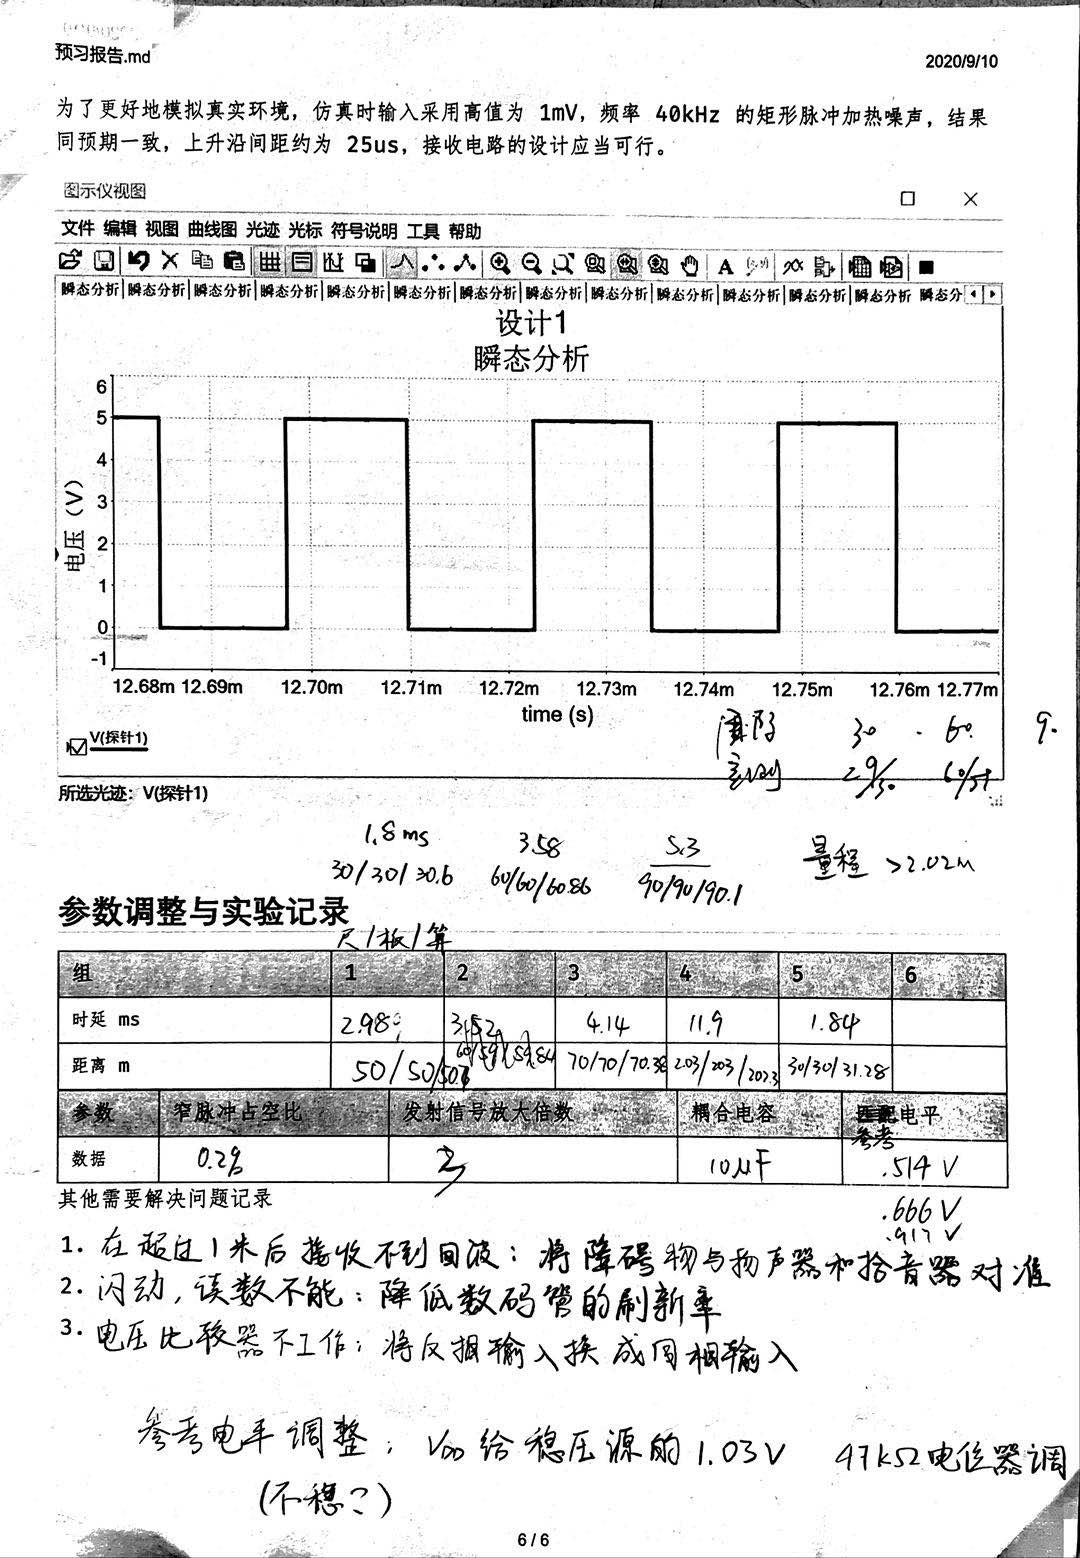
\includegraphics[width=7.5cm]{../assets/数据1.jpg}}
    \subfigure{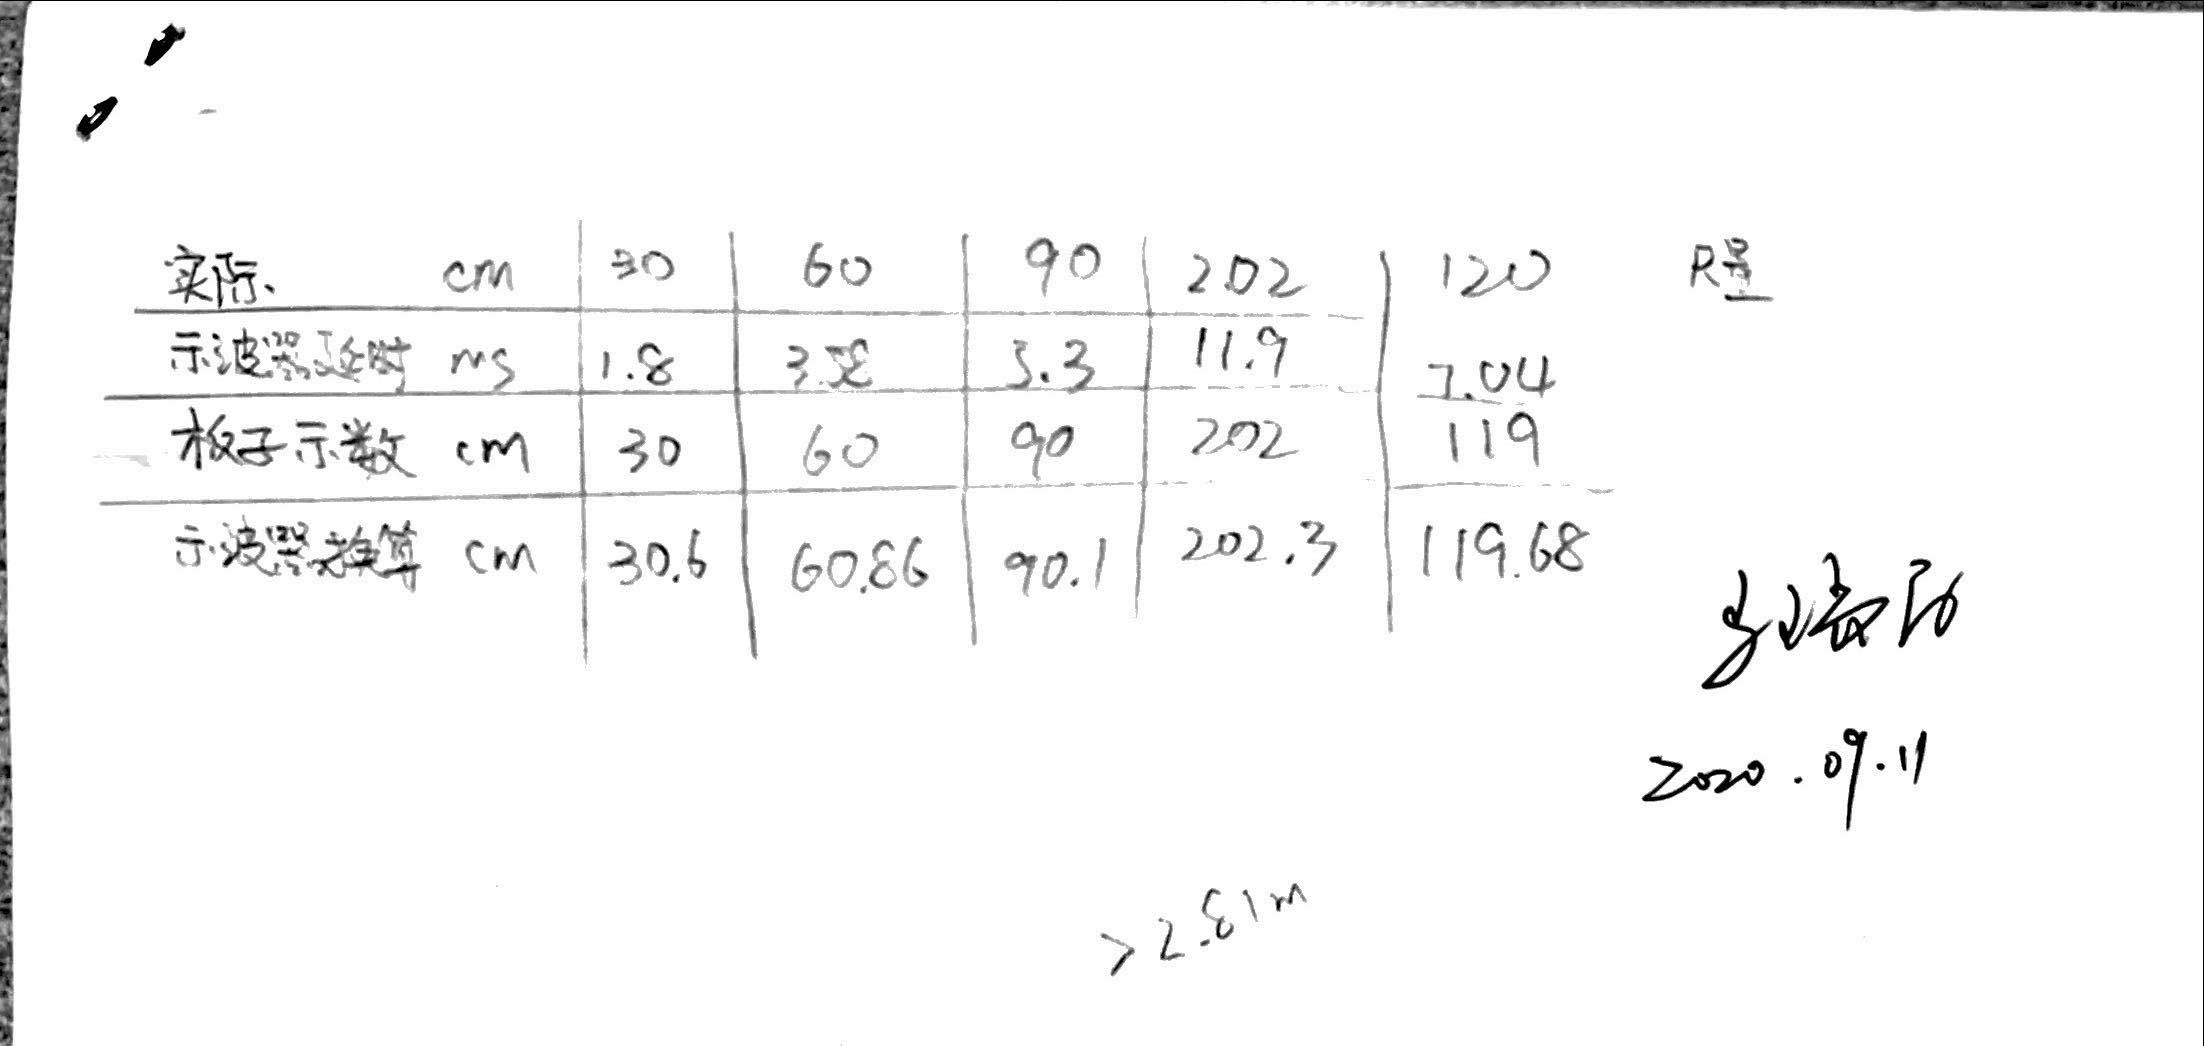
\includegraphics[width=7.5cm]{../assets/数据2.jpg}}
\end{figure}

\section{成本分析}

表\ref{tab:cost}为本实验中使用元器件数量及价格。

\begin{table}[h]
    \centering
    \caption{实验所用元器件数量及价格}
    \label{tab:cost}
    \begin{tabular}{ccc}
        \toprule
        元器件    & 数量(个) & 价格(元)                 \\
        \midrule
        电阻电容  & 9        & 0.9                      \\
        TI LF347N & 1        & 1.8                      \\
        CD40106   & 1        & 0.3                      \\
        电源      & 1        & 20                       \\
        电位器    & 1        & 2.5                      \\
        EGO1 FPGA & 1        & 9.228\textsuperscript{*} \\
        \bottomrule
    \end{tabular}
\end{table}

*:EGO1 FPGA开发板平均占用率为2.6367\%,折算价格为$350 * 2.6367\% = 9.228$(元)。

\begin{figure}[h]
    \centering
    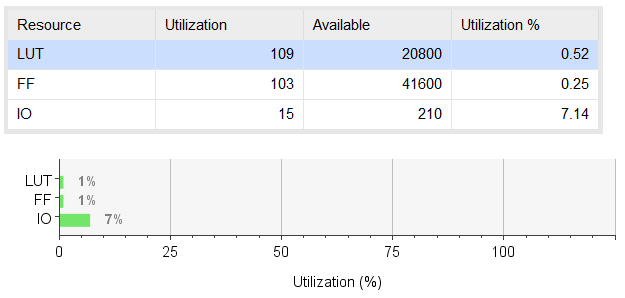
\includegraphics[width=7.5cm]{../assets/utilization.png}
    \caption{FPGA占用率}
\end{figure}

\end{document}